\addcontentsline{toc}{chapter}{Занятие 4. Оценка максимального правдоподобия}
\chapter*{Занятие 4. Оценка максимального правдоподобия}

\addcontentsline{toc}{section}{Контрольные вопросы и задания}
\section*{Контрольные вопросы и задания}

\subsubsection*{Как построить оценку максимального правдоподобия?}

Плотность распределения выборки $\left( X_1, \dotsc, X_n \right) $ имеет вид
$$L \left( \vec{X}, \theta \right) =
  \prod \limits_{k = 1}^n p \left( X_k, \theta \right),$$
как плотность вектора с независимыми координатами.
$L \left( \vec{X}, \theta \right) $ --- функция правдоподобия.

Оценка максимаьлного правдоподобия $ \hat{ \theta }$ --- такое значение параметра $ \theta $,
при котором функция правдоподобия достикает своего максимального значения
$ \hat{ \theta } =
  \underset{ \theta }{argmax} L \left( \vec{X}, \theta \right) $.

\subsubsection*{Сформулируйте свойства оценки максимального правдоподобия.}

Оценка максимального правдоподобия, как правило, сильно состоятельная.

\addcontentsline{toc}{section}{Аудиторные задачи}
\section*{Аудиторные задачи}

\subsubsection*{4.3}

\textit{Задание.}
Постройте оценку максимального правдоподобия векторного параметра $ \left( a, \sigma^2 \right) $
нормального распределения.

\textit{Решение.} Выборка $x_1, \dotsc, x_n \sim N \left( a, \sigma^2 \right) $.
Сейчас $ \theta $ будет векторным параметром, состоящим из двух элементов: $a, \sigma^2$.

Плотность имеет вид
$$p \left( x \right) =
  \frac{1}{ \sqrt{2 \pi } \sigma } \cdot e^{- \frac{ \left( x - a \right)^2}{2 \sigma^2}}.$$

Произведение этих плотностей даёт
$$L \left( \vec{x}, a, \sigma^2 \right) =
  \frac{1}{ \left( 2 \pi \right)^{ \frac{n}{2}} \sigma^n}
  \cdot e^{- \frac{1}{2 \sigma^n} \cdot \sum \limits_{i = 1}^n \left( x_i - a \right)^2}.$$
Обозначим $ \sigma^2 = \sigma^*$, чтобы было удобней брать производную
$$ \frac{1}{ \left( 2 \pi \right)^{ \frac{n}{2}} \sigma^2}
  \cdot e^{- \frac{1}{2 \sigma^2} \cdot \sum \limits_{i = 1}^n \left( x_i - a \right)^2} =
  \frac{1}{ \left( 2 \pi \right)^{ \frac{n}{2}} \left( \sigma^* \right)^{ \frac{n}{2}}} \cdot
  e^{- \frac{1}{2 \sigma^*} \cdot \sum \limits_{i = 1}^n \left( x_i - a \right)^2}.$$

Поскольку есть экспонента, стоит брать логарифм
$$l \left( \vec{x}, a, \sigma^* \right) =
  ln L \left( \vec{x}, a, \sigma^* \right) =
  - \frac{n}{2} \cdot ln \left( 2 \pi \sigma^* \right) -
  \frac{1}{2 \sigma^*} \sum \limits_{i = 1}^n \left( x_i - a \right)^2.$$
Распишем логарифм произведения через сумму логарифмов
$$- \frac{n}{2} \cdot ln \left( 2 \pi \sigma^* \right) -
  \frac{1}{2 \sigma^*} \sum \limits_{i = 1}^n \left( x_i - a \right)^2 =
  - \frac{n}{2} \cdot ln \left( 2 \pi \right) -
  \frac{n}{2} \cdot ln \sigma^* -
  \frac{1}{2 \sigma^*} \sum \limits_{i = 1}^n \left( x_i - a \right)^2.$$

Берём производную
$$ \frac{ \partial }{ \partial \sigma^*} l =
  - \frac{n}{2} \cdot \frac{1}{ \sigma^*} +
  \frac{1}{2 \left( \sigma^* \right)^2} \sum \limits_{i = 1}^n \left( x_i - a \right)^2 =
  0.$$

Теперь надо по $a$ продифференцировать и тоже приравнять к нулю
$$ \frac{ \partial }{ \partial a} l =
  \frac{1}{ \sigma^*} \sum \limits_{i = 1}^n \left( x_i - a \right) =
  0 =
  \frac{n \overline{X} - na}{ \sigma^*}.$$

Распишем сумму в явном виде
$ \left( x_1 - a \right) + \left( x_2 - a \right) + \dotsc + \left( x_n - a \right) =
  0$.

Отсюда
$$a =
  \frac{1}{n} \sum \limits_{i = 1}^n x_i.$$

Оценка равна $ \hat{a} = \overline{x}.$

Тогда оценка второго параметра равна
$$ \hat{ \sigma^*} =
  \frac{1}{n} \sum \limits_{i = 1}^n \left( x_i - \overline{x} \right)^2.$$

Проверили только необходимое условие для максимума.
Теперь нужно проверить достаточность.

Имеем матрицу $n \times n$.
Матрица положительно определена тогда и только тогда, когда каждый минор положительный.
Матрица отрицательно определена тогда и только тогда, когда каждый минор отрицательный.

$$ \begin{bmatrix}
  \frac{ \partial^2}{ \partial a^2} & \frac{ \partial^2}{ \partial a \partial \sigma^*} \\
  \frac{ \partial^2}{ \partial a \partial \sigma^*} & \frac{ \partial^2}{ \partial \left( \sigma^* \right)^2}
\end{bmatrix}.$$

Найдём последний элемент матрицы
$$ \frac{ \partial^2}{ \partial \left( \sigma^* \right)^2} l =
  \frac{n}{2 \left( \sigma^* \right)^2} -
  \frac{1}{ \left( \sigma^* \right)^3} \cdot \sum \limits_{i = 1}^n \left( x_i - a \right)^2.$$

Найдём смешанную производную
$$ \frac{ \partial^2}{ \partial a \partial \sigma^*} l =
  - \sum \limits_{i = 1}^n \left( x_i - a \right) \cdot \frac{1}{ \left( \sigma^* \right)^2} =
  \frac{n \overline{x} - na}{ \left( \sigma^* \right)^2}.$$

Найдём первый элемент матрицы
$$ \frac{ \partial^2}{ \partial a^2} l =
  - \frac{n}{ \sigma^*}.$$

Теорема Шварца.
Если
$$ \exists \frac{ \partial^2 f}{ \partial x \partial y}, \,
  \frac{ \partial^2 f}{ \partial y \partial x}$$
и они непрерывны в точке $ \left( x_0, y_0 \right) $, то они совпадают в этой точке.

Первый определитель строго отрицательный.

Второй определитель
$$M_2 =
  - \frac{n^2}{2 \left( \sigma^* \right)^3} +
  \frac{n}{ \left( \sigma^* \right)^4} \cdot \sum \limits_{i = 1}^n \left( x_i - a \right) -
  \frac{n}{ \left( \sigma^* \right)^4} \cdot \left( \overline{x} - a \right)^2.$$
Последнее слагаемое равно нулю.
Нужно проверять это значение в точке $ \hat{a} = \overline{x}$.
Имеем
\begin{equation*}
  \begin{split}
    - \frac{n^2}{2 \left( \sigma^* \right)^3} +
    \frac{n}{ \left( \sigma^* \right)^4} \cdot \sum \limits_{i = 1}^n \left( x_i - a \right) -
    \frac{n}{ \left( \sigma^* \right)^4} \cdot \left( \overline{x} - a \right)^2 = \\
    = - \frac{n}{ \left( \sigma^* \right)^3} \cdot
    \left( \frac{n}{2} - \frac{1}{ \sigma^*} \cdot
    \sum \limits_{i = 1}^n \left( x_i - a \right) \right) >
    0.
  \end{split}
\end{equation*}

Нужно проверить в точке $ \sigma^* = \hat{ \sigma }$.
Имеем
$$ \frac{n}{2} <
  \frac{ \sum \limits_{i = 1}^n \left( x_i - a \right)^2}{ \sigma^*}.$$

Отсюда выражаем значение оценки
$$ \sigma^* =
  \hat{ \sigma } =
  \frac{1}{n} \sum \limits_{i = 1}^n \left( x_i - \overline{x} \right).$$
Следовательно,
$$ \frac{n}{2} < n,$$
то есть $M_2 < 0$.
По критерию Сильвестра $ \hat{A} < 0$ тогда и только тогда,
когда $ \left( \hat{a}, \hat{ \sigma^*} \right) $ --- точка максимума.

\subsubsection*{4.5}

\textit{Задание.}
Постройте оценку максимального правдоподобия параметра $ \theta $ показательного распределения.

\textit{Решение.}
$p \left( x, \theta \right) =
  \theta e^{- \theta x} \cdot \mathbbm{1} \left\{ x \geq 0 \right\} $.

Нужно найти функцию правдобоподия как произведение плотностей
$L \left( \vec{x}, \theta \right) =
  \theta^n \cdot e^{-n \theta \sum \limits_{i = 1}^n x_i} \cdot
  \mathbbm{1} \left\{ \vec{x} \in \left[ 0, + \infty \right)^n \right\} $.
Предполагаем, что все $x_i \geq 0$, то есть индикатор можно отбросить.
Если какой-то элемент выборки сильно отрицательный,
то не имеет смысла говорить о равномерном распределении.
Если какой-то элемент выборки близок к нулю и при этом отрицательный, то на него повлияла ошибка,
и его не учитываем
$$ \theta^n \cdot e^{-n \theta \sum \limits_{i = 1}^n x_i} \cdot
  \mathbbm{1} \left\{ \vec{x} \in \left[ 0, + \infty \right)^n \right\} =
  \theta^n e^{-n \theta \sum \limits_{i = 1}^n x_i}.$$

Удобнее будет рассмотреть
$$ln L \left( \vec{x}, \theta \right) =
  l \left( \theta \right) =
  - \theta \sum \limits_{i = 1}^n x_i + n ln \theta.$$

Нужно взять производную и приравнять к нулю
$$ \frac{ \partial }{ \partial \theta } l \left( \theta \right) =
  - \sum \limits_{i = 1}^n x_i + \frac{n}{ \theta } =
  0.$$

Переносим сумму вправо
$$ \frac{n}{ \theta } =
  \sum \limits_{i = 1}^n x_i.$$

Получаем оценку
$$ \hat{ \theta } =
  \frac{n}{ \sum \limits_{i = 1}^n x_i}.$$
Выразим через выборочное среднее
$$ \frac{n}{ \sum \limits_{i = 1}^n x_i} =
  \frac{1}{ \overline{X}}.$$
Остаётся проверить, что $ \hat{ \theta }$ будет действительно максимумом функции $l$.
Нужно найти вторую производную
$$ \frac{ \partial^2}{ \partial \theta^2} l \left( \theta \right) =
  - \frac{n}{ \theta^n} <
  0.$$
Отсюда следует, что фунция выпуклая ввекх, соответственно это точка максимума.

\subsubsection*{4.6}

\textit{Задание.}
Постройте оценку максимального правдоподобия параметра $ \theta > 0$
равномерного распределения на отрезке $ \left[ 0, \theta \right] $.

\textit{Решение.}
Плотность равномерного распределения на отрезке $ \left[ 0, \theta \right] $ имеет вид
$$p_{ \theta } \left( x \right) =
  \frac{ \mathbbm{1} \left\{ x \in \left[ 0, \theta \right] \right\} }{ \theta }.$$
По этой плотности строим функцию правдоподобия
$$L \left( \vec{x}, \theta \right) =
  \frac{ \mathbbm{1} \left\{ \vec{x} \in \left[ 0, \theta \right]^n \right\} }{ \theta^n} =
  \frac{ \mathbbm{1} \left\{ \min \limits_i x_i \geq 0, \, \max \limits_i x_i \leq \theta \right\} }{ \theta^n}.$$
Если какой-то элемент выборки сильно отрицательный,
то не имеет смысла говорить о равномерном распределении, если близок к нулю,
то на него повлияла ошибка, и его не учитываем
$$ \frac{ \mathbbm{1} \left\{ \min \limits_i x_i \geq 0, \, \max \limits_i x_i \leq \theta \right\} }{ \theta^n} =
  \frac{ \mathbbm{1} \left\{ \max \limits_i x_i \leq \theta \right\} }{ \theta }.$$

Нарисуем график получившейся функции как функции от $ \theta $ (рис. \ref{fig:46}).

\begin{figure}[h!]
  \centering
  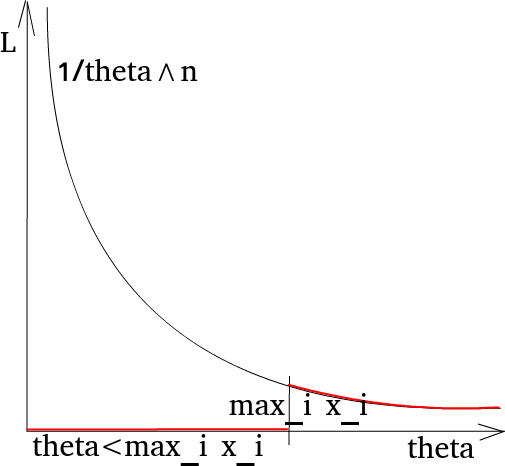
\includegraphics[width=.4\textwidth]{./pictures/4_6.png}
  \caption{График функции $L \left( \theta \right) $}
  \label{fig:46}
\end{figure}

Точка максимума такой функции --- это $ \max \limits_i x_i$.

Значит, $ \hat{ \theta } = \max \limits_{1 \leq i \leq n} x_i$.

\subsubsection*{4.7}

\textit{Задание.}
Постройте оценку максимального правдоподобия параметра сдвига $ \beta \in \mathbb{R}$
показательного распределения с плотностью
$$f_{ \beta } \left( y \right) =
  \begin{cases}
    e^{ \beta - y}, \qquad y \geq \beta, \\
    0, \qquad otherwise.
  \end{cases}$$

Проверьте состоятельность этой оценки.

\textit{Решение.}
$f_{ \beta } \left( y \right) = e^{ \beta - y} \cdot \mathbbm{1} \left\{ y \geq \beta \right\}.$

Запишем функцию правдоподобия
$$L \left( \vec{x}, \beta \right) =
  e^{n \beta - \sum \limits_{i = 1}^n x_i} \cdot
  \mathbbm{1} \left\{ \vec{x} \in \left[ \beta, + \infty \right)^n \right\} =
  e^{n \beta - \sum \limits_{i = 1}^n x_i} \cdot
  \mathbbm{1} \left\{ \min \limits_{1 \leq i \leq n} x_i \geq \beta \right\}.$$
Рисуем схематический график (рис. \ref{fig:47}).

\begin{figure}[h!]
  \centering
  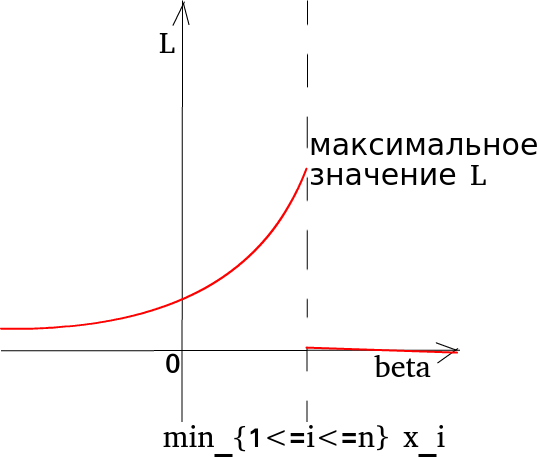
\includegraphics[width=.4\textwidth]{./pictures/4_7.png}
  \caption{График функции $L \left( \beta \right) $}
  \label{fig:47}
\end{figure}

Из графика видно, что $ \hat{ \beta } = \min \limits_{1 \leq i \leq n} x_i$.
Проверяем состоятельность:
$$ \hat{ \beta } \overset{P}{ \to } \beta, \, n \to \infty.$$
По определению
$P \left( \left| \hat{ \beta } - \beta \right| > \varepsilon \right) \to 0,
  \, n \to \infty, \,
  \forall \varepsilon > 0$.
Подставляем оценку в функцию правдоподобия
$$e^{n \beta - \sum \limits_{i = 1}^n x_i} \cdot
  \mathbbm{1} \left\{ \min \limits_{1 \leq i \leq n} x_i \geq \beta \right\} =
  P \left( \left| \min \limits_{1 \leq i \leq n} x_i - \beta \right| > \varepsilon \right).$$
Минимальный член выборки не может быть меньше $ \beta $ из-за распределения.
$P \left( \left| \min \limits_{1 \leq i \leq n} x_i - \beta \right| > \varepsilon \right) =
  P \left( \min \limits_{1 \leq i \leq n} x_i > \beta + \varepsilon \right).$
Запишем через вероятность пересечения событий $ \left\{ x_i > \beta + \varepsilon \right\} $.
Получим
$$P \left( \min \limits_{1 \leq i \leq n} x_i > \beta + \varepsilon \right) =
  P \left( \bigcap \limits_{i = 1}^n \left\{ x_i > \beta + \varepsilon \right\} \right).$$
Случайные величины независимы и одинаково распределены
$$P \left( \bigcap \limits_{i = 1}^n \left\{ x_i > \beta + \varepsilon \right\} \right) =
  \left[ P \left( x_1 > \beta + \varepsilon \right) \right]^n \to 0, \,
  n \to \infty,$$
так как такая вероятность меньше единицы.

Достаточно показать, что $P \left( x_1 > \beta + \varepsilon \right) \neq 1$.
Тогда $l^n \to 0$.

Запишем интеграл от плотности со сдвигом
$$ \int \limits_{ \beta + \varepsilon }^{+ \infty } p_{ \beta } \left( y \right) dy =
  1 - \int \limits_{ \beta }^{ \beta + \varepsilon } p_{ \beta } \left( y \right) dy <
  1,$$
так как второй интеграл больше нуля (забрали кусок $ \beta + \varepsilon $).

\subsubsection*{4.8}

\textit{Задание.}
Постройте оценку максимального правдоподобия параметра сдвига $ \mu \in \mathbb{R}$
распределения Лапласа с плотностью
$f_{ \mu } \left( y \right) =
  e^{- \frac{ \left| y - \mu \right| }{2}}$.

\textit{Решение.} Записываем функцию правдоподобия
$$L \left( \vec{X}, \mu \right) =
  \prod \limits_{i = 1}^n f_{ \mu } \left( X_i \right) =
  \prod \limits_{i = 1}^n \frac{1}{2} \cdot e^{- \left| X_i - \mu \right| } =
  \frac{1}{2^n} \cdot e^{- \sum \limits_{i = 1}^n \left| X_i - \mu \right| }.$$

Находим  логарифм
$$l \left( \vec{X}, \mu \right) =
  c - \sum \limits_{i = 1}^n \left| X_i - \mu \right|,$$
где $c = const$.
Дифференцировать по $ \mu $ не можем.
Хотим максимизировать эту функцию правдоподобия.
Нужно минимизировать сумму $X_i$ --- точки на оси.
$ \left| X_i - \mu \right| $ --- расстояние.

Вариационный ряд имеет понятие медианы.
Это приблизительно средина вариационного ряда.

$$ \mu^* =
  \begin{cases}
    X_{ \left( m + 1 \right) }, \qquad n = 2m + 1, \\
    \frac{X_{ \left( m \right) + X_{ \left( m + 1 \right) }}}{2}, \qquad n = 2m
  \end{cases}$$
--- аналогия с центром масс треугольника, который задаётся как точка пересечения медиан.

\subsubsection*{4.9}

\textit{Задание.} Постройте оценку максимального правдоподобия параметра $p$ распределения Бернулли.

\textit{Решение.} Распределение Бернулли не имеет плотности.
Есть выборка $x_1, \dotsc, x_n \sim B \left( 1, p \right) $.

Сформулируем метод максимального правдоподобия в общем случае.

$X_1, \dotsc, X_n$ --- выборка с параметром $ \theta $.

$X_1, \dotsc, X_n$ имеют плотность распределения $p_{ \theta } \left( y \right) $.
Тогда
$$L \left( \vec{X}, \theta \right) =
  \prod \limits_{i = 1}^n p_{ \theta } \left( X_i \right).$$
Отсюда находим $ \hat{ \theta } = argmax L \left( \vec{X}, \theta \right)$.

В дискретном случае плотность заменяем функцией $f \left( x \right) = P \left\{ Y = x \right\} $.

Имеем распределение $P \left( X = k \right) = p^k \cdot \left( 1 - p \right)^{1 - k}, \, k = 0, 1$.
Следовательно,
$$L \left( \vec{X}, p \right) =
  \prod \limits_{i = 1}^n p^{X_i} \left( 1 - p \right)^{1 - X_i} =
  p^{ \sum \limits_{i = 1}^n X_i} \cdot
  \left( 1 - p \right)^{ \sum \limits_{i = 1}^n \left( 1 - X_i \right) }=
  p^{n \overline{X}} \cdot \left( 1 - p \right)^{n \left( 1 - \overline{X} \right) }.$$
Функцию непрерывна по $p$.
Можем продифференцировать
$$l \left( \vec{X}, p \right) =
  n \overline{X} ln p + n \left( 1 - \overline{X} \right) ln \left( 1 - p \right).$$

Берём производную и приравниваем к нулю
$$ \frac{ \partial l}{ \partial p} =
  \frac{n \overline{X}}{p} - \frac{n \left( 1 - \overline{X} \right) }{1 - p} = 0.$$
Сокращаем на $n$ и переносим второе слагаемое вправо
$$ \frac{ \overline{X}}{p} =
  \frac{1 - \overline{X}}{1 - p}.$$
Перемножаем как пропорцию $ \overline{X} - p \overline{X} = p \left( 1 - \overline{X} \right) $.
Отсюда следует, что $p^* = \overline{X}$.

Проверим это, взяв вторую производную и посмотрев на её знак
$$ \frac{ \partial^2 l}{ \partial p^2} =
  - \frac{n \overline{X}}{p^2} -
  \frac{n \left( 1 - \overline{X} \right) }{ \left( 1 - p \right)^2} <
  0,$$
следовательно, $p^* = argmax l \left( \vec{X}, p \right) $.

\subsubsection*{4.10}

\textit{Задание.}
Пусть задана выборка из нормального распределения с единичной
дисперсией и математическим ожиданием $a$, которое может принимать только два значения: 1 или 2.
Постройте оценку максимального правдоподобия параметра $a$.

\textit{Решение.} Записываем общую функцию правдоподобия, как функцию параметра $a$.

Запишем для этого плотность распределения каждого элемента
$$p \left( x \right) =
  \frac{1}{ \sqrt{2 \pi }} \cdot e^{- \frac{ \left( x - a \right)^2}{2}}.$$
Теперь
$$L \left( \vec{X}, a \right) =
  \prod \limits_{i = 1}^n \frac{1}{ \sqrt{2 \pi }} \cdot e^{- \frac{ \left( X_i - a \right)^2}{2}} =
  \frac{1}{ \left( 2 \pi \right)^{ \frac{n}{2}}} \cdot
  e^{- \frac{1}{2} \sum \limits_{ \left( X_i - a \right)^2}}.$$

Записываем логарифм
$$l \left( \vec{X}, a \right) =
  - \frac{n}{2} \cdot ln \left( 2 \pi \right) -
  \frac{1}{2} \sum \limits_{i = 1}^n \left( X_i - a \right).$$

Подставим возможные значения $a$ и найдём разность логарифмов двух
соответствующих функций правдоподобия
$$l \left( \vec{X}, 2 \right) - l \left( \vec{X}, 1 \right) =
  \frac{1}{2} \sum \limits_{i = 1}^n \left( X_i - 2 \right)^2 -
  \frac{1}{2} \sum \limits_{i = 1}^n \left( X_i - 1 \right)^2.$$
Запишем под одну сумму
$$ \frac{1}{2} \sum \limits_{i = 1}^n \left( X_i - 2 \right)^2 -
  \frac{1}{2} \sum \limits_{i = 1}^n \left( X_i - 1 \right)^2 =
  \frac{1}{2} \cdot
  \sum \limits_{i = 1}^n \left[ \left( X_i - 2 \right)^2 - \left( X_i - 1 \right)^2 \right].$$
Разложим на 2 множителя
$$ \frac{1}{2} \cdot
  \sum \limits_{i = 1}^n \left[ \left( X_i - 2 \right)^2 - \left( X_i - 1 \right)^2 \right] =
  \frac{1}{2} \cdot
  \sum \limits_{i = 1}^n \left( X_i - 2 - X_i + 1 \right) \left( X_i - 2 + X_i - 1 \right).$$
Приведём подобные
$$ \frac{1}{2} \cdot
  \sum \limits_{i = 1}^n \left( X_i - 2 - X_i + 1 \right) \left( X_i - 2 + X_i - 1 \right) =
  \frac{1}{2} \sum \limits_{i = 1}^n \left( 2X_i - 3 \right) \left( -1 \right).$$
Выносим $n$ за скобки
$$ \frac{1}{2} \sum \limits_{i = 1}^n \left( 2X_i - 3 \right) \left( -1 \right) =
  n \left( \frac{3}{2} - \vec{X} \right).$$

Знак разности будет зависеть от значения $ \vec{X}$.

Если
$$ \vec{X} <
  \frac{3}{2},$$
то $a^* = 1$, если
$$ \vec{X} \geq
  \frac{3}{2},$$
то $a^* = 2$.

\addcontentsline{toc}{section}{Домашнее задание}
\section*{Домашнее задание}

\subsubsection*{4.14}

\textit{Задание.}
Постройте оценку максимального правдоподобия дисперсии $ \sigma^2$ нормального распределения,
если математическое ожидание $a$ известно.
Выясните, не является ли оценка состоятельной оценкой параметра $ \sigma^2$.

\textit{Решение.}
$$p_{ \sigma^2} \left( y \right) =
  \frac{1}{ \sqrt{2 \pi } \sigma } \cdot e^{- \frac{ \left( y - a \right)^2}{2 \sigma^2}}.$$

Запишем функцию правдоподобия
$$L \left( \vec{x}, \sigma^2 \right) =
  \frac{1}{ \left( 2 \pi \right)^{ \frac{n}{2}} \sigma^n} \cdot
  e^{- \frac{ \sum \limits_{i = 1}^n \left( x_i - a \right)^2}{2 \sigma^2}} =
  \frac{1}{ \left( 2 \pi \right)^{ \frac{n}{2}} \sigma^n} \cdot
  e^{- \frac{1}{2 \sigma^2} \cdot \sum \limits_{i = 1}^n \left( x_i - a \right)^2}.$$
Обозначим $ \sigma^2 = \sigma^*$, чтобы было удобнее брать производную
$$ \frac{1}{ \left( 2 \pi \right)^{ \frac{n}{2}} \sigma^n} \cdot
  e^{- \frac{1}{2 \sigma^2} \cdot \sum \limits_{i = 1}^n \left( x_i - a \right)^2} =
  \frac{1}{ \left( 2 \pi \sigma^* \right)^{ \frac{n}{2}}} \cdot
  e^{- \frac{1}{2 \sigma^*} \cdot \sum \limits_{i = 1}^n \left( x_i - a \right)^2}.$$

Поскольку есть экспонента, стоит брать логарифм
$$l \left( \vec{x}, \sigma^2 \right) =
  ln L \left( \vec{x}, \sigma^2 \right) =
  - \frac{n}{2} \cdot ln \left( 2 \pi \sigma^* \right) -
  \frac{1}{2 \sigma^*} \sum \limits_{i = 1}^n \left( x_i - a \right)^2.$$
Распишем логарифм произведения через сумму логарифмов в первом слагаемом
$$- \frac{n}{2} \cdot ln \left( 2 \pi \sigma^* \right) -
  \frac{1}{2 \sigma^*} \sum \limits_{i = 1}^n \left( x_i - a \right)^2 =
  - \frac{n}{2} \cdot ln \left( 2 \pi \right) -
  \frac{n}{2} \cdot ln \sigma^* -
  \frac{1}{2 \sigma^*} \sum \limits_{i = 1}^n \left( x_i - a \right)^2.$$

Берём производную и приравниваем её к нулю
$$ \frac{ \partial l}{ \partial \sigma^*} =
  - \frac{n}{2} \cdot \frac{1}{ \sigma^*} +
  \frac{1}{2 \left( \sigma^* \right)^2} \sum \limits_{i = 1}^n \left( x_i - a \right)^2 =
  0.$$

Выносим в знаменателе $ \sigma^*$ за скобку, сокращаем и переносим первое слагаемое вправо
$$ \frac{1}{2 \sigma^*} \sum \limits_{i = 1}^n \left( x_i - a \right)^2 =
  \frac{n}{2}.$$

Выражаем оценку
$$ \sigma^* =
  \hat{ \sigma^2} =
  \frac{ \sum \limits_{i = 1}^n \left( x_i - a \right)^2}{n}.$$

Проверили необходимое условие для максимума.
Теперь нужно проверить достаточное.

Найдём вторую производную
$$ \frac{ \partial^2 l}{ \partial \left( \sigma^* \right)^2} =
  \frac{ \partial }{ \partial \sigma^*}
    \left[
      - \frac{n}{2} \cdot \frac{1}{ \sigma^*} +
      \frac{1}{2 \left( \sigma^* \right)^2} \sum \limits_{i = 1}^n \left( x_i - a \right)^2
    \right] =
  \frac{n}{2 \left( \sigma^* \right)^2} -
  \frac{1}{ \left( \sigma^* \right)^3} \cdot \sum \limits_{i = 1}^n \left( x_i - a \right)^2.$$
Подставим найденное значение оценки
$$ \frac{n}{2 \left( \sigma^* \right)^2} -
  \frac{1}{ \left( \sigma^* \right)^3} \cdot \sum \limits_{i = 1}^n \left( x_i - a \right)^2 =
  \frac{n \cdot n^2}{2 \left[ \sum \limits_{i = 1}^n \left( x_i - a \right)^2 \right]^2} -
  \frac{n^3}{ \left[ \sum \limits_{i = 1}^n \left( x_i - a \right)^2 \right]^3} \cdot
  \sum \limits_{i = 1}^n \left( x_i - a \right)^2.$$
Упростим
\begin{equation*}
  \begin{split}
    \frac{n \cdot n^2}{2 \left[ \sum \limits_{i = 1}^n \left( x_i - a \right)^2 \right]^2} -
    \frac{n^3}{ \left[ \sum \limits_{i = 1}^n \left( x_i - a \right)^2 \right]^3} \cdot
    \sum \limits_{i = 1}^n \left( x_i - a \right)^2 = \\
    = \frac{n^3}{2 \left[ \sum \limits_{i = 1}^n \left( x_i - a \right)^2 \right]^2} -
    \frac{n^3}{ \left[ \sum \limits_{i = 1}^n \left( x_i - a \right)^2 \right]^2} =
    \frac{n^3}{ \left[ \sum \limits_{i = 1}^n \left( x_i - a \right)^2 \right]^3} \cdot
    \left( \frac{1}{2} - 1 \right) = \\
    = - \frac{n^3}{2 \left[ \sum \limits_{i = 1}^n \left( x_i - a \right)^2 \right]^3} <
    0,
  \end{split}
\end{equation*}
следовательно, $ \hat{ \sigma^2}$ --- точка максимума функции.
Проверим состоятельность, то есть $ \hat{ \sigma^2} \overset{P}{ \to } \sigma^2, \, n \to \infty $.

По закону больших чисел
$$ \frac{1}{n} \sum \limits_{i = 1}^n \left( x_i - a \right)^2 \overset{P}{ \to }
  M \left( x_1 - a \right)^2 =
  Dx_1 =
  \sigma^2, \,
  n \to \infty,$$
то есть оценка состоятельная.

\subsubsection*{4.15}

\textit{Задание.}
Постройте оценку максимального правдоподобия параметра $ \lambda > 0$ распределения Пуассона.

\textit{Решение.} Распределение Пуассона не имеет плотности.
Есть выборка $x_1, \dotsc, x_n \sim Pois \left( \lambda \right), \, \lambda > 0$.

Функция правдоподобия, когда есть плотность, выглядит так
$$L \left( \vec{x}, \lambda \right) =
  \prod \limits_{i = 1}^n p_{ \lambda } \left( x_i \right).$$

Введём функцию
$f_{ \lambda } \left( x \right) =
  P \left\{ x_1 = x \right\} =
  P \left\{ \left. \omega \right| x_1 \left( \omega \right) = x \right\} $,
где
$$x \in
  \left\{ 0, 1, \dotsc \right\}.$$

В этом случае функция правдоподобия примет вид
$$L \left( \vec{x}, \lambda \right) =
  \prod \limits_{i = 1}^n f_{ \lambda } \left( x_i \right).$$

Ищем максимум функции правдоподобия.
Нужно записать
$$f_{ \lambda } \left( x \right) =
  \frac{ \lambda^x}{x!} \cdot e^{- \lambda }.$$

Подставляем в функцию правдоподобия
$$ \prod \limits_{i = 1}^n f_{ \lambda } \left( x_i \right) =
  \prod \limits_{i = 1}^n \left( \frac{ \lambda^{x_i}}{x_i!} \cdot e^{- \lambda } \right) =
  \frac{ \lambda^{ \sum \limits_{i = 1}^n x_i}}{ \prod \limits_{i = 1}^n x_i!} \cdot
  e^{- \lambda n}.$$

Так как есть экспонента, возьмём логарифм
$$l \left( \vec{x}, \lambda \right) =
  ln L \left( \vec{x}, \lambda \right) =
  ln \left(
    \frac{ \lambda^{ \sum \limits_{i = 1}^n x_i}}{ \prod \limits_{i = 1}^n x_i!} \cdot
    e^{- \lambda n}
  \right) =
  - \lambda n + \sum \limits_{i = 1}^n x_i \cdot ln \lambda - ln \prod \limits_{i = 1}^n x_i!.$$

Берём производную по $ \lambda $, приравниваем её к нулю
$$ \frac{ \partial l \left( \vec{x}, \lambda \right) }{ \partial \lambda } =
  -n + \sum \limits_{i = 1}^n x_i \cdot \frac{1}{ \lambda } =
  0.$$

Ищем оценку
$$ \sum \limits_{i = 1}^n x_i \cdot \frac{1}{ \lambda } =
  n,$$
откуда
$$ \lambda^* =
  \frac{ \sum \limits_{i = 1}^n x_i}{n} =
  \overline{x}.$$

Проверили необходимое условие максимума.
Проверим достаточное,
то есть найдём вторую производную логарифма функции правдоподобия и посмотрим на её знак
$$ \frac{ \partial^2 l \left( \vec{x}, \lambda \right) }{ \partial \lambda^2} =
  \frac{ \partial }{ \partial \lambda } \left(
    -n + \sum \limits_{i = 1}^n x_i \cdot \frac{1}{ \lambda }
  \right) =
  \sum \limits_{i = 1}^n x_i \cdot \frac{ \partial \lambda^{-1}}{ \partial \lambda } =
  - \sum \limits_{i = 1}^n x_i \cdot \frac{1}{ \lambda^2} <
  0,$$
то есть точка $ \lambda^* = \overline{x}$ --- точка максимума функции правдоподобия,
то есть оценка максимального правдоподобия.

\subsubsection*{4.16}

\textit{Задание.}
Постройте оценку максимального прадоподобия параметра
$$p \in
  \left(0, 1 \right) $$
геометрического распределения.

\textit{Решение.} Геометрическое распределение не имеет плотности.

Сформирулируем метод максимального правдоподобия в общем случае.

$X_1, \dotsc, X_n$ --- выборка с параметром $ \theta $.

Случайные величины $X_1, \dotsc, X_n$ имеют плотность распределения
$p_{ \theta } \left( y \right) $.
Тогда
$$L \left( \vec{X}, \theta \right) =
  \prod \limits_{i = 1}^n p_{ \theta } \left( X_i \right).$$

Отсюда находим $ \hat{ \theta } = argmax L \left( \vec{X}, \theta \right) $.

В дискретном случае плотность заменяется функцией $f \left( x \right) = P \left\{ Y = x \right\} $.

Имеем распределение $P \left( X = k \right) = p \left( 1 - p \right)^k$, где $k = 0, 1, 2, \dotsc $.
Следовательно,
$$L \left( \vec{X}, p \right) =
  \prod \limits_{i = 1}^n p \left( 1 - p \right)^{X_i} =
  p^n \left( 1 - p \right)^{ \sum \limits_{i = 1}^n X_i}  =
  p^n \left( 1 - p \right)^{n \overline{X}}.$$

Функция непрерывна по $p$, можем дифференцировать.

$l \left( \vec{X}, p \right) =
  nlnp + n \overline{X} ln \left( 1 - p \right) $.

Берём производную и приравниваем к нулю
$$ \frac{ \partial l}{ \partial p} =
  \frac{n}{p} - \frac{n \overline{X} }{1 - p} =
  0.$$
Сокращаем на $n$ и переновим второе слагаемое вправо
$$ \frac{1}{p} =
  \frac{ \overline{X}}{1 - p}.$$

Перемножаем как пропорцию $1 - p = p \overline{X}$.
Отсюда слудует, что
$$1 =
  p + p \overline{X} =
  p \left( 1 + \overline{X} \right),$$
и
$$p^* =
  \frac{1}{1 + \overline{X}}.$$

Проверим это, взяв вторую производную и посмотрев на её знак
$$ \frac{ \partial^2 l}{ \partial p^2} =
  - \frac{n}{p^2} - \frac{n \overline{X}}{ \left( 1 - p \right)^2} <
  0,$$
следовательно, $p^* = argmax l \left( \vec{X}, p \right) $.

\subsubsection*{4.17}

\textit{Задание.}
Пусть задана выборка из биномиального распределения с параметрами $p \in \left( 0, 1 \right) $ и
$m$.
Постройте оценку максимального правдоподобия параметра:
\begin{enumerate}[label=\alph*)]
  \item $p$, если значение параметра $m$ известно;
  \item $m$ по выборке объёма $n = 1$, если значение $p$ известно.
\end{enumerate}

\textit{Решение.} Биномиальное распределение не имеет плотности.

Сформирулируем метод максимального правдоподобия в общем случае.

$X_1, \dotsc, X_n$ --- выборка с параметром $ \theta $.

Случайные величины $X_1, \dotsc, X_n$ имеют плотность распределения
$p_{ \theta } \left( y \right) $.
Тогда
$$L \left( \vec{X}, \theta \right) =
  \prod \limits_{i = 1}^n p_{ \theta } \left( X_i \right).$$

Отсюда находим $ \hat{ \theta } = argmax L \left( \vec{X}, \theta \right) $.

В дискретном случае плотность заменяется функцией $f \left( x \right) = P \left\{ Y = x \right\} $.

Имеем распределение
$P \left( X = k \right) = C_m^k p^k \left( 1 - p \right)^{m - k}, \,
  k = \overline{0, m}$.
Следовательно,
$$L \left( \vec{X}, p, m \right) =
  \prod \limits_{i = 1}^n C_m^{X_i} p^{X_i} \left( 1 - p \right)^{m - X_i} =
  \prod \limits_{i = 1}^n C_m^{X_i} \cdot
  p^{ \sum \limits_{i = 1}^n X_i} \cdot
  \left( 1 - p \right)^{ \sum \limits_{i = 1}^n \left( m - X_i \right) }.$$
Записываем через выборочное среднее
$$ \prod \limits_{i = 1}^n C_m^{X_i} \cdot
  p^{ \sum \limits_{i = 1}^n X_i} \cdot
  \left( 1 - p \right)^{ \sum \limits_{i = 1}^n \left( m - X_i \right) } =
  \prod \limits_{i = 1}^n C_m^{X_i} \cdot
  p^{n \overline{X}} \left( 1 - p \right)^{n \left( m - \overline{X} \right) }.$$

\begin{enumerate}[label=\alph*)]
  \item Функция непрерывна по $p$.
  Можем дифференцировать.

  $l \left( \vec{X}, p, m \right) =
    \sum \limits_{i = 1}^n C_m^{X_i} +
    n \overline{X} ln p +
    n \left( m - \overline{X} \right) ln \left( 1 - p \right) $.

  Берём производную и приравниваем к нулю
  $$ \frac{ \partial l}{ \partial p} =
    \frac{n \overline{X}}{p} - \frac{n \left( m - \overline{X} \right) }{1 - p} = 0.$$

  Сокращаем на $n$ и переносим вправо второе слагаемое
  $$ \frac{ \overline{X}}{p} =
    \frac{m - \overline{X}}{1 - p}.$$

  Перемножим как пропорцию $ \overline{X} - p \overline{X} = p \left( m - \overline{X} \right) $.
  Отсюда следует, что $p \left( m - \overline{X} \right) + p \overline{X} = \overline{X}$,
  и оценка равна
  $$p^* =
    \frac{ \overline{X}}{m - \overline{X} + \overline{X}} =
    \frac{ \overline{X}}{m}.$$

  Проверим это, взяв вторую производную и посмотрев на её знак
  $$ \frac{ \partial^2 l}{ \partial p^2} =
    - \frac{m \overline{X}}{p^2} -
    \frac{m \left( m - \overline{X} \right) }{ \left( 1 - p \right)^2} <
    0,$$
  следовательно, $p^* = argmax \, l \left( \vec{X}, p \right) $;
  \item в данном случае $ \vec{X} = X_1$.
  Имеем функцию правдоподобия
  $$L_m =
    C_m^{X_1} p^{X_1} \left( 1 - p \right)^{m - X_1} =
    L \left( X_1, m \right) =
    L \left( \vec{X}, m \right),$$
  соответственно $L_{m - 1} = C_{m - 1}^{X_1} p^{X_1} \left( 1 - p \right)^{m - 1 - X_1}$.

  Найдём отношение
  $$ \frac{L_m}{L_{m - 1}} =
    \frac{C_m^{X_1} p^{X_1} \left( 1 - p \right)^{m - X_1}}{C_{m - 1}^{X_1} p^{X_1} \left( 1 - p \right)^{m - 1 - X_1}} =
    \frac{m! \left( 1 - p \right) X_1 ! \left( m - X_1 - 1 \right)!}{X_1 ! \left( m - X_1 \right)! \left( m - 1 \right)!}.$$
  Сокращаем факториалы
  $$ \frac{m! \left( 1 - p \right) X_1 ! \left( m - X_1 - 1 \right)!}{X_1 ! \left( m - X_1 \right)! \left( m - 1 \right)!} =
    \frac{m \left( 1 - p \right) }{m - X_1}.$$

  Возможны 2 случая
  $$ \begin{cases}
    \frac{m \left( 1 - p \right) }{m - X_1} \geq 1, \\
    \frac{m \left( 1 - p \right) }{m - X_1} \leq 1.
  \end{cases}$$
  Переносим знаменатель вправо
  $$ \begin{cases}
    m \left( 1 - p \right) \geq m - X_1, \\
    m \left( 1 - p \right) \leq m - X_1.
  \end{cases}$$
  Переносим слагаемые с $m$ в одну сторону
  $$ \begin{cases}
    m - m \left( 1 - p \right) \leq X_1, \\
    m - m \left( 1 - p \right) \geq X_1.
  \end{cases}$$
  Выносим $m$ за скобки
  $$ \begin{cases}
    m \left( 1 - 1 + p \right) \leq X_1, \\
    m \left( 1 - 1 + p \right) \geq X_1.
  \end{cases}$$
  Получаем
  $$ \begin{cases}
    m \leq \frac{X_1}{p}, \\
    m \geq \frac{X_1}{p}.
  \end{cases}$$
  Отсюда оценка равна
  $$m^* =
    \left[ \frac{X_1}{p} \right].$$
\end{enumerate}

\subsubsection*{4.18}

\textit{Задание.}
Постройте оценку максимального правдоподобия параметра $ \theta $
равномерного распределения на отрезке:
\begin{enumerate}[label=\alph*)]
  \item $ \left[- \theta, 0 \right], \, \theta > 0$;
  \item $ \left[- \theta, \theta \right], \, \theta > 0$;
  \item $ \left[ \theta , \theta + 2 \right], \, \theta \in \mathbb{R}$;
  \item $ \left[ \theta, 2 \theta \right], \, \theta > 0$.
\end{enumerate}

\textit{Решение.}
\begin{enumerate}[label=\alph*)]
  \item Плотность равномерного распределения а отрезке $ \left[- \theta, 0 \right], \, \theta > 0$
  имеет вид
  $$p_{ \theta } \left( x \right) =
    \frac{1}{ \theta } \cdot \mathbbm{1} \left\{ x \in \left[ - \theta, 0 \right] \right\}.$$

  По этой плотности строим функцию правдоподобия
  $$L \left( \vec{x}, \theta \right) =
    \frac{ \mathbbm{1} \left\{ \vec{x} \in \left[ - \theta, 0 \right]^n \right\} }{ \theta^n} =
    \frac{ \mathbbm{1} \left\{ \min \limits_i x_i \geq - \theta, \, \max \limits_i x_i \leq 0 \right\} }{ \theta ^n}.$$
  Если какой-то элемент выборки сильно положительный,
  то не имеет смысла говорить о равномерном распределении, если положительный, но близок к нулю,
  то на него повлияла ошибка, и его не учитываем
  $$ \frac{ \mathbbm{1} \left\{ \min \limits_i x_i \geq - \theta, \, \max \limits_i x_i \leq 0 \right\} }{ \theta ^n} =
    \frac{ \mathbbm{1} \left\{ \min \limits_i x_i \geq - \theta \right\} }{ \theta^n}.$$

  Нарисуем график получившейся функции, как функции от $ \theta $ (рис. \ref{fig:418}).
  \begin{figure}[h!]
    \centering
    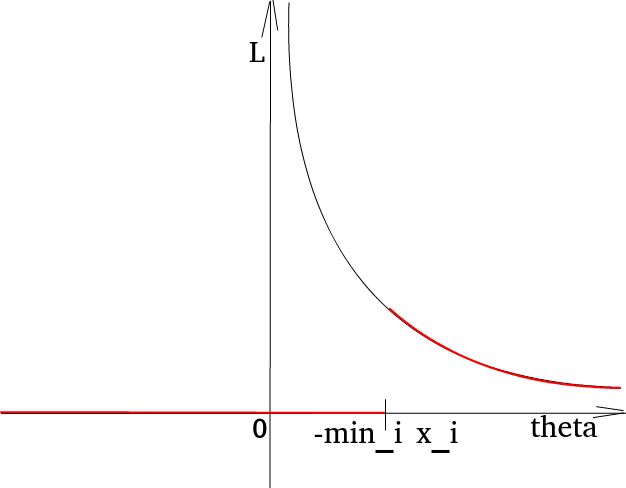
\includegraphics[width=.4\textwidth]{./pictures/4_18.png}
    \caption{График функции $L \left( \theta \right) $}
    \label{fig:418}
  \end{figure}

  Точка максимума этой функции --- это $ \left( - \min \limits_i x_i \right) $.

  Значит, $ \hat{ \theta } = - \min \limits_{1 \leq i \leq n} x_i$;
  \item плотность равномерного распределения на отрезке
  $ \left[- \theta, \theta \right], \, \theta > 0$ имеет вид
  $$p_{ \theta } \left( x \right) =
    \frac{ \mathbbm{1} \left\{ x \in \left[ - \theta, \theta \right] \right\} }{2 \theta }.$$

  По этой функции строим функцию правдоподобия
  $$L \left( \vec{x}, \theta \right) =
    \frac{ \mathbbm{1} \left\{ \vec{x} \in \left[ - \theta, \theta \right]^n \right\} }{ \left( 2 \theta \right)^n} =
    \frac{ \mathbbm{1} \left\{ \min \limits_i x_i \geq - \theta, \, \max \limits_i x_i \leq \theta \right\} }{ \left( 2 \theta \right)^n}.$$
  Меняем знак для минимального элемента выборки
  $$ \frac{ \mathbbm{1} \left\{ \min \limits_i x_i \geq - \theta, \, \max \limits_i x_i \leq \theta \right\} }{ \left( 2 \theta \right)^n} =
    \frac{1}{ \left( 2 \theta \right)^n} \cdot
    \mathbbm{1} \left\{
      \max \limits_i x_i \leq \theta, \, - \min \limits_i x_i \leq \theta
    \right\}.$$
  Берём максимум
  \begin{equation*}
    \begin{split}
      \frac{1}{ \left( 2 \theta \right)^n} \cdot
      \mathbbm{1} \left\{
        \max \limits_i x_i \leq \theta, \, - \min \limits_i x_i \leq \theta
      \right\} = \\
      = \frac{1}{ \left( 2 \theta \right)^n} \cdot
      \mathbbm{1} \left\{
        \max \left( \max \limits_i x_i, \, - \min \limits_i x_i \right) \leq \theta
      \right\}.
    \end{split}
  \end{equation*}

  Нарисуем график этой функции, как функции от $ \theta $ (рис. \ref{fig:4181}).

  \begin{figure}[h!]
    \centering
    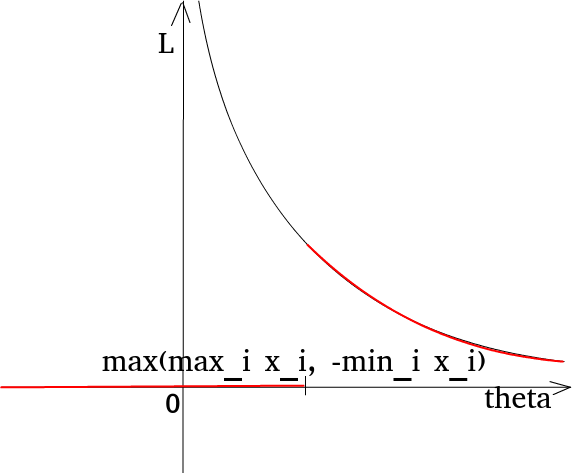
\includegraphics[width=.4\textwidth]{./pictures/4_18_1.png}
    \caption{График функции $L \left( \theta \right) $}
    \label{fig:4181}
  \end{figure}

  Точка максимума такой функции ---
  это $ \max \left( \max \limits_i x_i, \, - \min \limits_i x_i \right) $.

  Значит,
  $ \hat{ \theta } =
    \max \left(
      \max \limits_{1 \leq i\leq n} x_i, \, - \min \limits_{1 \leq i \leq n} x_i
    \right) $;
  \item плотность равномерного распределения на отрезке
  $ \left[ \theta , \theta + 2 \right], \, \theta \in \mathbb{R}$ имеет вид
  $$p_{ \theta } \left( x \right) =
    \frac{ \mathbbm{1} \left\{ x \in \left[ \theta, \theta + 2 \right] \right\} }{2}.$$

  По этой плотности строим функцию правдоподобия
  $$L \left( \vec{x}, \theta \right) =
    \frac{ \mathbbm{1} \left\{ \vec{x} \in \left[ \theta, \theta + 2 \right]^n \right\} }{2^n} =
    \frac{ \mathbbm{1} \left\{ \min \limits_i x_i \geq \theta, \, \max \limits_i x_i \leq \theta + 2 \right\} }{2^n}.$$
  Переносим 2 влево
  $$ \frac{ \mathbbm{1} \left\{ \min \limits_i x_i \geq \theta, \, \max \limits_i x_i \leq \theta + 2 \right\} }{2^n} =
    \frac{ \mathbbm{1} \left\{ \min \limits_i x_i \geq \theta, \, \max \limits_i x_i - 2 \leq \theta \right\} }{2^n}.$$
  Значит,
  $ \max \limits_{1 \leq i \leq n} x_i - 2 \leq
    \hat{ \theta } \leq
    \min \limits_{1 \leq i \leq n} x_i$;
  \item плотность равномерного распределения на отрезке
  Значит, $ \max \limits_{1 \leq i \leq n} x_i - 2 \leq \hat{ \theta } \leq \min \limits_{1 \leq i \leq n} x_i$;
  $ \left[ \theta, 2 \theta \right], \, \theta > 0$ имеет вид
  $$p_{ \theta } \left( x \right) =
    \frac{ \mathbbm{1} \left\{ x \in \left[ \theta, 2 \theta \right] \right\} }{ \theta }.$$

  По этой функции строим функцию правдоподобия
  $$L \left( \vec{x}, \theta \right) =
    \frac{ \mathbbm{1} \left\{ \vec{x} \in \left[ \theta, 2 \theta \right]^n \right\} }{ \theta^n} =
    \frac{ \mathbbm{1} \left\{ \min \limits_i x_i \geq \theta, \, \max \limits_i x_i \leq 2 \theta \right\} }{ \theta^n}.$$
  Делим неравенство с максимумом на 2
  $$ \frac{ \mathbbm{1} \left\{ \min \limits_i x_i \geq \theta, \, \max \limits_i x_i \leq 2 \theta \right\} }{ \theta^n} =
    \frac{ \mathbbm{1} \left\{ \min \limits_i x_i \geq \theta,\, \frac{ \max \limits_i x_i}{2} \leq \theta \right\} }{ \theta^n}.$$
  Остюда следует, что
  $$ \frac{ \max \limits_i x_i}{2} \leq
    \theta \leq
    \min \limits_i x_i.$$

  Нарисуем график полученной функции, как функции от $ \theta $ (рис. \ref{fig:4183}).

  \begin{figure}[h!]
    \centering
    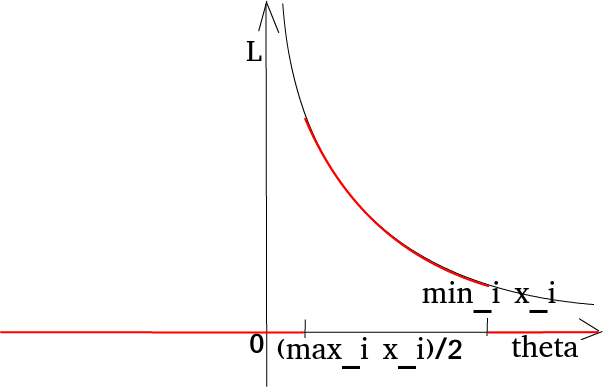
\includegraphics[width=.4\textwidth]{./pictures/4_18_3.png}
    \caption{График функции $L \left( \theta \right) $}
    \label{fig:4183}
  \end{figure}

  Точка максимума такой функции --- это
  $$ \frac{ \max \limits_i x_i}{2}.$$

  Значит,
  $$ \hat{ \theta } =
    \frac{ \max \limits_{1 \leq i \leq n} x_i}{2}.$$
\end{enumerate}

\subsubsection*{4.19}

\textit{Задание.}
Пусть $X_1, \dotsc, X_n$ ---
выборка из друхпараметрического показательного распределения с плотностью
$$f_{ \alpha, \beta } \left( y \right) =
  \begin{cases}
    \alpha^{-1} e^{- \frac{y - \beta }{ \alpha }}, \qquad y \geq \beta, \\
    0, \qquad otherwise,
  \end{cases}$$
где $ \alpha > 0, \, \beta \in \mathbb{R}$.
Постройте оценку максимального правдоподобия двумерного параметра $ \left( \alpha, \beta \right) $.
Проверьте состоятельность этой оценки.

\textit{Решение.}
Сейчас $ \theta $ будет векторным параметром, состоящим из двух элементов: $ \alpha, \beta $.

Плотность имеет вид
$$f_{ \alpha, \beta } \left( y \right) =
  \frac{1}{ \alpha } \cdot
  e^{- \frac{y}{ \alpha } + \frac{ \beta }{ \alpha }} \cdot
  \mathbbm{1} \left\{ y \geq \beta \right\}.$$

Произведение этих плотностей даёт
$$L \left( \vec{X}, \alpha, \beta \right) =
  \frac{1}{ \alpha^n} \cdot
  e^{- \frac{1}{ \alpha } \sum \limits_{i = 1}^n \left( X_i - \beta \right) } \cdot
  \mathbbm{1} \left\{ \vec{X} \in \left[ \beta, + \infty \right)^n \right\}.$$
Все элементы выборки не меньше, чем $ \beta $.
Запишем это условие через минимальный элемент
$$ \frac{1}{ \alpha^n} \cdot
  e^{- \frac{1}{ \alpha } \sum \limits_{i = 1}^n \left( X_i - \beta \right) } \cdot
  \mathbbm{1} \left\{ \vec{X} \in \left[ \beta, + \infty \right)^n \right\} =
  \frac{1}{ \alpha^n} \cdot
  e^{- \frac{1}{ \alpha } \sum \limits_{i = 1}^n \left( X_i - \beta \right) }
  \cdot \mathbbm{1} \left\{ \min \limits_{1 \leq i \leq n} X_i \geq \beta \right\}.$$

Найдём $ \beta^*$.
При фиксированном $ \alpha $ нарисуем график функции правдоподобия как функции от $ \beta $
(рис. \ref{fig:419}).

\begin{figure}[h!]
  \centering
  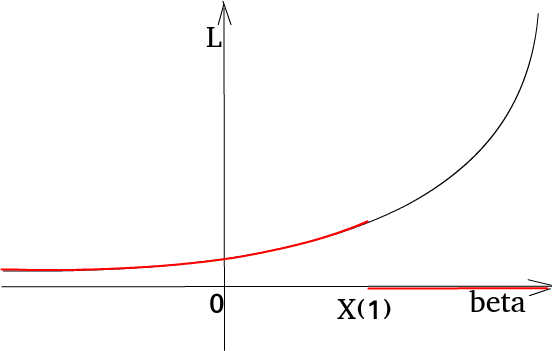
\includegraphics[width=.4\textwidth]{./pictures/4_19.png}
  \caption{График функции $L \left( \beta \right) $}
  \label{fig:419}
\end{figure}

Из графика видно, что точка максимума этой функции ---
это точка $ \min \limits_{1 \leq i \leq n} X_i = \beta^*$.

Так как есть экспонента, удобнее взять логарифм от функции правдоподобия
$$ln \left( \vec{X}, \alpha, \beta \right) =
  l \left( \vec{X}, \alpha, \beta \right) =
  -n ln \alpha + \frac{n \beta - \sum \limits_{i = 1}^n X_i}{ \alpha }.$$

Возьмём производную по $ \alpha $ и приравняем её к нулю
$$ \frac{ \partial l}{ \partial \alpha } =
  -n \cdot \frac{1}{ \alpha } - \frac{n \beta - \sum \limits_{i = 1}^n X_i}{ \alpha^2} =
  0.$$
Умножим на $ \left( - \alpha^2 \right) $ левую и правую части уравнения
$$n \alpha + n \beta - \sum \limits_{i = 1}^n X_i =
  0.$$

Отсюда выражаем оценку
$$ \alpha^* =
  \frac{1}{n} \sum \limits_{i = 1}^n X_i - \beta^* =
  \overline{X} - \min \limits_{1 \leq i \leq n} X_i.$$

Проверим состоятельность.
Нужно проверить,
выполняется ли
$$ \left( \alpha^*, \beta^* \right) \overset{P}{ \to } \left( \alpha , \beta \right), \,
  n \to \infty.$$

По определению
$P \left( \left| \beta^* - \beta \right| > \varepsilon \right) \to 0, \,
  n \to \infty, \,
  \forall \varepsilon > 0$.

Подставим в вероятность оценку
$$P \left( \left| \beta^* - \beta \right| > \varepsilon \right) =
  P \left( \left| \min \limits_{1 \leq i \leq n} X_i - \beta \right| > \varepsilon \right).$$

Из распределения $ \min \limits_{1 \leq i \leq n} X_i \geq \beta $, следовательно,
можем убрать модуль
$P \left( \left| \min \limits_{1 \leq i \leq n} X_i - \beta \right| > \varepsilon \right) =
  P \left( \min \limits_{1 \leq i \leq n} X_i - \beta > \varepsilon \right) =
  P \left( \min \limits_{1 \leq i \leq n} X_i > \beta + \varepsilon \right) = \\
  = P \left( \bigcap \limits_{i = 1}^n \left\{ X_i > \beta + \varepsilon \right\} \right) $.
Случайные величины независимые и одинаково распределённые
$P \left( \bigcap \limits_{i = 1}^n \left\{ X_i > \beta + \varepsilon \right\} \right) =
  \left[ P \left( X_1 > \beta + \varepsilon \right) \right]^n \to 0, \,
  n \to \infty,$
так как $P \left( X_1 > \beta + \varepsilon \right) \neq 1$.

Значит, $ \beta^*$ --- состоятельная оценка.
Тогда по закону больших чисел
$$ \alpha^* =
  \frac{1}{n} \sum \limits_{i = 1}^n X_i - \beta^* \overset{P}{ \to }
  MX_1 - \beta =
  \int \limits_{ \beta }^{+ \infty }
    \frac{1}{ \alpha } \cdot e^{- \frac{-y}{ \alpha }} e^{ \frac{ \beta }{ \alpha }} ydy -
  \beta. $$
Возьмём интеграл по частям
$$u = y, \,
  du = dy, \,
  dv = e^{- \frac{y}{ \alpha }} dy, \,
  v = \int e^{- \frac{y}{ \alpha }} dy = - \alpha e^{- \frac{y}{ \alpha }}.$$
Получим
$$ \int \limits_{ \beta }^{+ \infty }
    \frac{1}{ \alpha } \cdot e^{- \frac{-y}{ \alpha }} e^{ \frac{ \beta }{ \alpha }} ydy -
  \beta =
  \left.
    \frac{1}{ \alpha } \cdot
    e^{ \frac{ \beta }{ \alpha }} \left( - \alpha \right) y e^{- \frac{y}{ \alpha }}
  \right|_{ \beta }^{+ \infty } +
  \frac{1}{ \alpha } \cdot e^{ \frac{ \beta }{ \alpha }} \cdot \alpha \cdot
  \int \limits_{ \beta }^{+ \infty } e^{- \frac{y}{ \alpha }} dy -
  \beta.$$
Подставим пределы интегрирования и возьмём интеграл
$$ \left.
    \frac{1}{ \alpha } \cdot
    e^{ \frac{ \beta }{ \alpha }} \left( - \alpha \right) y e^{- \frac{y}{ \alpha }}
  \right|_{ \beta }^{+ \infty } +
  \frac{1}{ \alpha } \cdot e^{ \frac{ \beta }{ \alpha }} \cdot \alpha \cdot
  \int \limits_{ \beta }^{+ \infty } e^{- \frac{y}{ \alpha }} dy -
  \beta =
  e^{ \frac{ \beta }{ \alpha }} \beta \cdot e^{- \frac{ \beta }{ \alpha }} -
  e^{ \frac{ \beta }{ \alpha }} \cdot
  \left. \alpha e^{- \frac{y}{ \alpha }} \right|_{ \beta }^{+ \infty } -
  \beta.$$
Сократим экспоненты и подставим пределы интегрирования во втором слагаемом
$$e^{ \frac{ \beta }{ \alpha }} \beta \cdot e^{- \frac{ \beta }{ \alpha }} -
  e^{ \frac{ \beta }{ \alpha }} \cdot
  \left. \alpha e^{- \frac{y}{ \alpha }} \right|_{ \beta }^{+ \infty } -
  \beta =
  \beta + \alpha e^{ \frac{ \beta }{ \alpha }} \cdot e^{- \frac{ \beta }{ \alpha }} - \beta =
  \alpha.$$

Получили, что оценка $ \alpha^*$ --- тоже состоятельная.

\subsubsection*{4.20}

\textit{Задание.} Пусть задана выборка из двухпараметричного распределения Лапласа с плотностью
$$f_{ \mu, \sigma} \left( y \right) =
  \frac{e^{- \frac{ \left| y - \mu \right| }{ \sigma }}}{2 \sigma }, \,
  \mu \in \mathbb{R}, \,
  \sigma > 0.$$

Постройте оценку максимального правдоподобия двумерного параметра $ \left( \mu, \sigma \right) $.

\textit{Решение.} Записываем функцию правдоподобия
$$L \left( \vec{X}, \mu, \sigma \right) =
  \prod \limits_{i = 1}^n f_{ \mu, \sigma } \left( X_i \right) =
  \prod \limits_{i = 1}^n
    \frac{1}{2 \sigma } \cdot e^{- \frac{ \left| X_i - \mu \right| }{ \sigma }} =
  \frac{1}{ \left( 2 \sigma \right)^n} \cdot
  e^{- \frac{1}{ \sigma } \sum \limits_{i = 1}^n \left| X_i - \mu \right| }.$$

Находим логарифм
$$l \left( \vec{X}, \mu, \sigma \right) =
  -n \, ln \left(2 \sigma \right) -
  \frac{1}{ \sigma } \sum \limits_{i = 1}^n \left| X_i - \mu \right| =
  - n \, ln 2 -
  n \, ln \sigma -
  \frac{1}{ \sigma } \sum \limits_{i = 1}^n \left| X_i - \mu \right|.$$
Дифференцировать по $ \mu $ не можем.
Хотим максимизировать функцию правдоподобия.
Нужно минимизировать сумму $X_i$ --- точки на оси.
$ \left| X_i - \mu \right| $ --- расстояние.

Вариационный ряд имеет понятие медианы.
Это приблизительно средина вариационного ряда
$$ \mu^* =
  \begin{cases}
    X_{ \left( m + 1 \right) }, \qquad n = 2m + 1, \\
    \frac{X_{ \left( m \right) + X_{ \left( m + 1 \right) }}}{2}, \qquad n = 2m
  \end{cases}$$
--- аналог с центром масс треугольника, который задаётся как точка пересечения медиан.

Найдём оценку второго параметра.
Нужно взять производную и приравнять к нулю
$$ \frac{ \partial l \left( \vec{X}, \mu, \sigma \right) }{ \partial \sigma } =
  - \frac{n}{ \sigma } + \frac{1}{ \sigma^2} \sum \limits_{i = 1}^n \left| X_i - \mu \right| =
  \frac{1}{ \sigma } \cdot
  \left( \frac{1}{ \sigma } \sum \limits_{i = 1}^n \left| X_i - \mu \right| - n \right) =
  0.$$

Приравниваем выражение в скобках к нулю
$$ \frac{1}{ \sigma } \sum \limits_{i =1}^n \left| X_i - \mu \right| =
  n.$$

Отсюда оценка равна
$$ \sigma^* =
  \frac{ \sum \limits_{i = 1}^n \left| X_i - \mu^* \right| }{n} =
  \left| \overline{X - \mu^*} \right|.$$
